%!TeX root=../tese.tex
%("dica" para o editor de texto: este arquivo é parte de um documento maior)
% para saber mais: https://tex.stackexchange.com/q/78101/183146

% Apague as duas linhas abaixo (elas servem apenas para gerar um
% aviso no arquivo PDF quando não há nenhum dado a imprimir) e
% insira aqui o conteúdo dos capítulos do seu trabalho

%!TeX root=../tese.tex
%("dica" para o editor de texto: este arquivo é parte de um documento maior)
% para saber mais: https://tex.stackexchange.com/q/78101/183146

%% ------------------------------------------------------------------------- %%
\chapter{Introdução}
\label{cap:introducao}
\section{Motivação}

A dificuldade em um jogo tende a ser um elemento extremamente visível e importante para o seu aproveitamento. Jogos mais desafiadores são conhecidos por serem mais frustrantes, e os menos desafiadores, mais relaxantes. Porém, esse pensamento pode levar à falsa idéia de impossibilitação do aproveitamento por parte da dificuldade elevada. No artigo de Jesper~\citet{FearOfFailing} é discutido o verdadeiro papel da dificuldade em jogos, de forma enxuta e didática. Quando apresentamos o conceito de vitória em um jogo, não faria sentido termos este sem o conceito de derrota. A derrota entra na experiência do jogo de forma a induzir os jogadores a reajustarem sua perspectiva perante ao jogo, como visto no estudo de Juul, levando o jogador a sempre pensar em novas estratégias e, consequentemente, adicionando conteúdo ao jogo.

O nivel de dificuldade de um jogo pode ser visto como o responsável pelo desenvolvimento nas habilidades do jogador em experimentos como o de~\citet{ExperimentalValidation}, porém, neste mesmo experimento, vemos ela também influenciando fortemente o aproveitamento geral do jogo, e podendo prejudicá-lo se não definida apropriadamente. Segundo~\citet{VideoGameBusiness}, jogos são uma das formas de entretenimento mais consumidas atualmente, totalizando uma receita de 159.3 bilhões de dólares no mundo inteiro em 2020. Portanto é natural associarmos jogos a entretenimento e, consequentemente, imaginarmos que um dado jogo é divertido, porém adequar a dificuldade de um jogo à experiência desejada prova-se um trabalho difícil.

escrever mais aqui
\textquotedbl{aspa}\textquotedbl{}

\section{Objetivos}

Considerando a tese apresentada, é necessário manter em mente que um jogador pode se sentir \textquotedbl{violado}\textquotedbl{} pelo jogo se este sofre mudanças drásticas em sua dificuldade durante ou entre as sessões jogadas~\citep{DynamicDiffAdjustment}. Com isso, foi almeijado um sistema onde ocorrem ajustes dinâmicos de dificuldade em um jogo, porém de forma a se adaptar ao nível da habilidade do jogador. Isso é, se o jogador se adapta bem à dificuldade atual do jogo, esta tende a aumentar, propondo um desafio adequado à habilidade do jogador. Em contrapartida, se o jogador é muito prejudicado pela dificuldade atual do jogo, esta tende a diminuir, com o fim de manter o jogador em um estado mais favorável à sua habilidade, mas que também o força a adaptar suas estratégias e seu estilo de jogo, permitindo-o \textquotedbl{avançar}\textquotedbl{} na dificuldade de jogo.

Escrever bem é uma arte que exige muita técnica e dedicação e,
consequentemente, há vários bons livros sobre como escrever uma boa
dissertação ou tese. Um dos trabalhos pioneiros e mais conhecidos nesse
sentido é o livro de
%Umberto Eco~\cite{eco:09} % usando o estilo alpha
Umberto~\citet{eco:09} % usando o estilo plainnat
intitulado \emph{Como se faz uma tese}; é uma leitura bem interessante mas,
como foi escrito em 1977 e é voltado para trabalhos de graduação na Itália,
não se aplica tanto a nós.

Sobre a escrita acadêmica em geral, John Carlis disponibilizou um texto curto
e interessante~\citep{carlis:09} em que advoga a preparação de um único
rascunho da tese antes da versão final. Mais importante que isso, no
entanto, são os vários \textit{insights} dele sobre a escrita acadêmica.
Dois outros bons livros sobre o tema são \emph{The Craft of Research}~\citep{craftresearch}
e \emph{The Dissertation Journey}~\citep{dissertjourney}. Além disso, a USP
tem uma compilação de normas relativas à produção de documentos
acadêmicos~\citep{usp:guidelines} que pode ser utilizada como referência.

Para a escrita de textos especificamente sobre Ciência da Computação, o
livro de Justin Zobel, \emph{Writing for Computer Science}~\citep{zobel:04}
é uma leitura obrigatória. O livro \emph{Metodologia de Pesquisa para
Ciência da Computação} de
%Raul Sidnei Wazlawick~\cite{waz:09} % usando o estilo alpha
Raul Sidnei~\citet{waz:09} % usando o estilo plainnat
também merece uma boa lida. Já para a área de Matemática, dois livros
recomendados são o de Nicholas Higham, \emph{Handbook of Writing for
Mathematical Sciences}~\citep{Higham:98} e o do criador do \TeX{}, Donald
Knuth, juntamente com Tracy Larrabee e Paul Roberts, \emph{Mathematical
Writing}~\citep{Knuth:96}.

Apresentar os resultados de forma simples, clara e completa é uma tarefa que
requer inspiração. Nesse sentido, o livro de
%Edward Tufte~\cite{tufte01:visualDisplay}, % usando o estilo alpha
Edward~\citet{tufte01:visualDisplay}, % usando o estilo plainnat
\emph{The Visual Display of Quantitative Information}, serve de ajuda na
criação de figuras que permitam entender e interpretar dados/resultados de forma
eficiente.

Além desse material, também vale muito a pena a leitura do trabalho de
%Uri Alon \cite{alon09:how}, % usando o estilo alpha
Uri \citet{alon09:how}, % usando o estilo plainnat
no qual apresenta-se uma reflexão sobre a utilização da Lei de Pareto para
tentar definir/escolher problemas para as diferentes fases da vida acadêmica.
A direção dos novos passos para a continuidade da vida acadêmica deveria ser
discutida com seu orientador.

%% ------------------------------------------------------------------------- %%
\section{Considerações de Estilo}
\label{sec:consideracoes_preliminares}

Normalmente, as citações não devem fazer parte da estrutura sintática da
frase\footnote{E não se deve abusar das notas de rodapé.\index{Notas de rodapé}}.
No entanto, usando referências em algum estilo autor-data (como o estilo
plainnat do \LaTeX{}), é comum que o nome do autor faça parte da frase. Nesses
casos, pode valer a pena mudar o formato da citação para não repetir o nome do
autor; no \LaTeX{}, isso pode ser feito usando os comandos
\textsf{\textbackslash{}citet}, \textsf{\textbackslash{}citep},
\textsf{\textbackslash{}citeyear} etc. documentados no pacote
natbib \citep{natbib}\index{natbib} (esses comandos são compatíveis com biblatex
usando a opção \textsf{natbib=true}, ativada por padrão neste modelo). Em geral,
portanto, as citações devem seguir estes exemplos:

\footnotesize
\begin{verbatim}
Modos de citação:
indesejável: [AF83] introduziu o algoritmo ótimo.
indesejável: (Andrew e Foster, 1983) introduziram o algoritmo ótimo.
certo: Andrew e Foster introduziram o algoritmo ótimo [AF83].
certo: Andrew e Foster introduziram o algoritmo ótimo (Andrew e Foster, 1983).
certo (\citet ou \citeyear): Andrew e Foster (1983) introduziram o algoritmo ótimo.
\end{verbatim}
\normalsize

O uso desnecessário de termos em língua estrangeira deve ser evitado. No entanto,
quando isso for necessário, os termos devem aparecer \textit{em itálico}.
\index{Língua estrangeira}
% index permite acrescentar um item no indice remissivo

Uma prática recomendável na escrita de textos é descrever as
legendas\index{Legendas} das figuras e tabelas em forma auto-contida: as
legendas devem ser razoavelmente completas, de modo que o leitor possa entender
a figura sem ler o texto onde a figura ou tabela é citada.\index{Floats}

Sugerimos que você faça referências bibliográficas de forma similar aos
estilos ``alpha'' (referências alfanuméricas) ou ``plainnat'' (referências
por autor-data) de \LaTeX{}.  Se estiver usando natbib+bibtex\index{natbib}\index{bibtex},
use os arquivos .bst ``alpha-ime.bst'' ou ``plainnat-ime.bst'', que são
versões desses dois formatos traduzidas para o português. Se estiver usando
biblatex\index{biblatex} (recomendado), escolha o estilo ``alphabetic''
(que é um dos estilos padrão do biblatex) ou ``plainnat-ime''. O arquivo de
exemplo inclui todas essas opções; basta des-comentar as linhas
correspondentes e, se necessário, modificar o arquivo Makefile para chamar
o bibtex\index{bibtex} ao invés do biber\index{biber} (este último é usado
em conjunto com o biblatex).

\section{Ferramentas Bibliográficas}

Embora seja possível pesquisar por material acadêmico na Internet usando sistemas
de busca ``comuns'', existem ferramentas dedicadas, como o \textsf{Google Scholar}\index{Google Scholar}
(\url{scholar.google.com}). Você também pode querer usar o \textsf{Web of Science}\index{Web of Science}
(\url{webofscience.com}) e o \textsf{Scopus}\index{Scopus} (\url{scopus.com}), que oferecem
recursos sofisticados e limitam a busca a periódicos com boa reputação acadêmica.
Essas duas plataformas não são gratuitas, mas os alunos da USP têm acesso a elas
através da instituição. Ambas são capazes de exportar os dados para o formato .bib,
usado pelo \LaTeX{}. Algumas editoras, como a ACM e a IEEE, também têm sistemas de
busca bibliográfica.

Apenas uma parte dos artigos acadêmicos de interesse está disponível livremente
na Internet; os demais são restritos a assinantes. A CAPES assina um grande
volume de publicações e disponibiliza o acesso a elas para diversas universidades
brasileiras, entre elas a USP, através do seu portal de periódicos
(\url{periodicos.capes.gov.br}). Existe uma extensão para os navegadores
Chrome e Firefox (\url{www.infis.ufu.br/capes-periodicos}) que facilita o uso
cotidiano do portal.

Para manter um banco de dados organizado sobre artigos e outras fontes bibliográficas
relevantes para sua pesquisa, é altamente recomendável que você use uma ferramenta
como Zotero~(\url{zotero.org})\index{Zotero} ou
Mendeley~(\url{mendeley.com})\index{Mendeley}. Ambas podem exportar seus dados no
formato .bib, compatível com \LaTeX{}. Também existem três plataformas
gratuitas que permitem a busca de referências acadêmicas já no formato .bib:

\begin{itemize}
  \item \emph{CiteULike}\index{CiteULike} (patrocinados por Springer): \url{www.citeulike.org}
  \item Coleção de bibliografia em Ciência da Computação: \url{liinwww.ira.uka.de/bibliography}
  \item Google acadêmico\index{Google Scholar} (habilitar bibtex nas preferências): \url{scholar.google.com}
\end{itemize}

Lamentavelmente, ainda não existe um mecanismo de verificação ou validação das
informações nessas plataformas. Portanto, é fortemente sugerido validar todas
as informações de tal forma que as entradas bib estejam corretas.

De qualquer modo, tome muito cuidado na padronização das referências
bibliográficas: ou considere TODOS os nomes dos autores por extenso, ou TODOS
os nomes dos autores abreviados.  Evite misturas inapropriadas.

\section{O Que o IME Espera}

Ao terminar sua tese/dissertação, você deve entregar uma cópia dela para a
CPG. Após a defesa, você tem 30 dias para revisar o texto e incorporar as
sugestões da banca. Assim, há duas versões oficiais do documento: a versão
original e a versão corrigida, o que deve ser indicado na folha de rosto.
\index{Tese/Dissertação!versões}

Fica a critério do aluno definir aspectos como o tamanho de fonte, margens,
espaçamento, estilo de referências, cabeçalho, etc. considerando sempre o
bom senso. A CPG, em reunião realizada em junho de 2007, aprovou que as
teses/dissertações deverão seguir o formato padrão por ela
definido\footnote{\url{www.ime.usp.br/dcc/pos/normas/tesesedissertacoes}}.
Esse padrão refere-se aos itens que devem estar presentes nas teses/dissertações
(e.g. capa, formato de rosto, sumário, etc.), e não à formatação do documento.
Ele define itens obrigatórios e opcionais, conforme segue:\index{Formatação}
\index{Tese/Dissertação!itens obrigatórios}
\index{Tese/Dissertação!itens opcionais}

\begin{itemize}
  \item \textsc{Capa} (obrigatória)
  \begin{itemize}
    \item O IME usa uma capa padrão de cartolina para todas as
    teses/dissertações.  Essa capa tem uma janela recortada por onde se
    vê o título e o autor do trabalho e, portanto, a capa impressa do
    trabalho deve incluir o título e o autor na posição correspondente da
    página. Ela fica centralizada na página, tem 100mm de largura, 60mm de
    altura e começa 47mm abaixo do topo da página.

    \item O título da tese/dissertação deverá começar com letra maiúscula
    e o resto deverá ser em minúsculas, salvo nomes próprios.

    \item O nome do aluno(a) deverá ser completo e sem abreviaturas.

    \item É preciso explicitar se é uma tese ou dissertação (para
    obtenção do título de doutor, tese; para obtenção do título de
    mestre, dissertação).

    \item O nome do programa deve constar da capa (Matemática,
    Matemática Aplicada, Estatística ou Ciência da Computação).

    \item Também devem constar o nome completo do orientador e do
    co-orientador, se houver.

    \item Se o aluno recebeu bolsa, deve-se indicar a(s) agência(s).

    \item É preciso informar o mês e ano do depósito ou da entrega da
    versão corrigida.
  \end{itemize}

  \item \textsc{Folha de Rosto} (obrigatória, tanto para a versão
  depositada quanto para a versão corrigida)
  \begin{itemize}
    \item o título da tese/dissertação deverá seguir o padrão da capa

    \item deve informar se se trata da versão original ou da versão
    corrigida; no segundo caso, deve também incluir os nomes
    dos membros da banca.
  \end{itemize}

  \item \textsc{Agradecimentos} (opcional)

  \item \textsc{Resumo}, em português (obrigatório)

  \item \textsc{Abstract}, em inglês (obrigatório)

  \item \textsc{Sumário} (obrigatório)

  \item \textsc{Listas} (opcionais)
  \begin{itemize}
    \item Lista de Abreviaturas
    \item Lista de Símbolos
    \item Lista de Figuras
    \item Lista de Tabelas
  \end{itemize}

  \item \textsc{Referências Bibliográficas} (obrigatório)

  \item \textsc{Índice Remissivo} (opcional\footnote{O índice remissivo
   pode ser muito útil para a banca; assim, embora seja um item opcional,
   recomendamos que você o crie.})
\end{itemize}

\par

%!TeX root=../tese.tex
%("dica" para o editor de texto: este arquivo é parte de um documento maior)
% para saber mais: https://tex.stackexchange.com/q/78101/183146

%% ------------------------------------------------------------------------- %%
\chapter{Dificuldade e Gêneros de Jogos}
\label{cap:dificuldade e generos de jogos}
\section{Arcades e Consoles}

\textit{Arcades}, mais comumente conhecidos como \textit{Fliperamas}, foram introduzidas na década de 1930, com jogos mecânicos ainda hoje famosos, como \textit{Pinball}. As máquinas eram projetadas com uma entrada de moeda, que quando inserida permitia que fossem jogados determinado número de vezes (\textquotedbl{rounds}\textquotedbl{} ou \textquotedbl{vidas}\textquotedbl{}). Não se afastando desse sistema, os jogos eletrônicos em gabinetes foram introduzidos apenas na década de 60 às \textit{Arcades}. Como relatado por~\citet{ArcadeGaming}, jogos como \textit{Pac-Man}, \textit{Donkey Kong}, \textit{Space Invaders}, \textit{Asteroids} e diversos outros títulos dominavam as \textit{Arcades} no mundo inteiro.

A partir desse ponto, foram apenas introduzidas novas tecnologias aos jogos de \textit{Arcade}. \textit{Duck Hunt} foi considerado revolucionário por usar um controle no formato  de um revólver, usado para mirar diretamente na tela, simulando um tiro-ao-alvo. Alguns anos depois, jogos de corrida como \textit{Grand Prix} levaram desenvolvedores à ideia de um controle no formato de um volante e um pedal, simulando, similarmente ao \textit{Duck Hunt}, um cenário de pilotagem mais próximo da realidade.

Por mais atraentes que os jogos de \textit{Arcade} estavam se tornando, sua dificuldade tendia a surpreender mais ainda o jogador. Até este momento, o papel principal da dificuldade era de se aproveitar ao máximo do sistema de moedas do jogo. Quanto mais difícil o jogo, mais moedas seriam gastas para completá-lo, e poucos desenvolvedores deixavam de ver essa vantagem.

Com a entrada dos \textit{consoles}\footnote{
    Aparelho dedicado a rodar um determinado grupo de jogos, com hardwares de interface (ex.: Playstation 2, Nintendo GameBoy, Xbox360).
}, principalmente do \textit{Nintendo Entertainment System}, também conhecido como \textit{NES} e \textit{Nintendinho}, jogos começaram a ser reestruturados, deixando de ter apenas uma fase e seu objetivo de arrecadar o maior número de pontos possível, e adquirindo uma estrutura mais linear, com diversas fases e, consequentemente, tendo seu objetivo principal deslocado para terminar todas as fases, ou derrotar o último chefe. Com isso, o papel da dificuldade sofreu uma leve mudança, deixando de buscar as moedas do jogador, e passando a ser a sustentação principal do tempo de jogo. Quanto mais difícil, mais tempo o jogador levaria para terminar o jogo, portanto maior aproveitamento seria tirado. Ideologias como essa moldaram a grande maioria dos jogos de \textit{NES} como jogos extremamente difíceis de se completar.

\section{Cenário Atual}

Após uma onda de jogos notoriamente difíceis, desenvolvedores começaram a explorar a ideia de dificuldades selecionáveis em jogos, em busca de poderem atender públicos mais abrangentes com seus projetos. Estava então emergindo a mecânica de, ao começar um \textit{novo jogo}, era apresentada a opção de dificuldade, normalmente variando entre \textit{fácil}, \textit{médio} e \textit{difícil}, mas não se limitando a essas opções.

Variáveis do jogo como quantidade de pontos de vida do jogador e dos inimigos oscilavam de acordo com a dificuldade escolhida. Os primeiros grandes jogos de sucesso a explorar mais a fundo a mecânica de diversos níveis de dificuldade, como \textit{Halo}, \textit{Call of Duty}, saga \textit{The Elder Scrolls}, saga \textit{Final Fantasy}, entre outros, moldaram esse padrão para uma grande parcela dos jogos futuros, porém não a perfeccionando instantaneamente. Picos na dificuldade eram comumente encontrados em níveis mais altos no jogo. As últimas dificuldades, normalmente rotuladas como \textit{Impossível} ou termos do gênero, costumavam inflar exageradamente variáveis do jogo como pontos de vida dos inimigos, muitas vezes tornando o jogo praticamente impossível e distanciando o jogador do cenário de entretenimento que os desenvolvedores se propunham a oferecer.

Em paralelo, é possível observar certas estruturas de jogos que permitem ao jogador explorar suas mecânicas de modo a afetar a dificuldade. Por exemplo, jogos no estilo \textit{Online Multiplayer}\footnote{
    Em contrapartida ao \textit{Singleplayer}, é um estilo de jogo onde diversas pessoas jogam uma partida juntas, em tempo real, através de seus respectivos aparelhos ou \textit{consoles} e uma conexão à \textit{internet}.
}, jogadores frequentemente participam de partidas e deliberadamente evitam usar certos itens do jogo, de modo a propor um desafio maior a si mesmos, se exibir ou até mesmo estabelecer recordes. Neste último cenário, também vemos a grande presença das \textit{Speedruns} em jogos \textit{Singleplayer}. Estas consistem em o jogador tentar completar determinado jogo no período de tempo mais curto possível. Para isso, o jogo é estudado profundamente e suas estratégias são otimizadas, procurando pular fases, explorar pontos fracos de inimigos ou até mesmo \textit{bugs} nos jogos. Essa cultura é popularmente conhecida por propor tarefas de dificuldade significativamente mais elevadas que o jogo \textquotedbl{base}\textquotedbl{}, consequentemente demandando muito da habilidade do jogador, ao mesmo tempo que adiciona conteúdo ao jogo.

Com o decorrer das décadas de 2000 e 2010, desenvolvedores começaram a aprofundar a complexidade do balanceamento da dificuldade de seus jogos~\citep{Zork:81}. A introdução de \textit{checkpoints}\footnote{
    Quando encontrado, garante que o jogador possa voltar a este ponto do jogo após ser derrotado. Funciona normalmente como uma \textquotedbl{volta no tempo}\textquotedbl{} para não punir tão severamente o jogador.
} tornou jogos extensos muito mais acessíveis~\citep{GameTime}, por impedir que a derrota levasse o jogador de volta para o primeiro nível do jogo, e reduzindo o quanto do jogo teria que ser rejogado. Jogos mais datados são conhecidos por praticamente não possuírem checkpoints, o que contribuia fortemente para sua dificuldade elevada. É importante, porém, manter em mente que um uso excessivo de \textit{checkpoints} pode trivializar as conquistas do jogador, uma vez que este não será apropriadamente punido por seus erros.

Neste mesmo período, com o avanço das Inteligências Artificiais (IAs), jogos \textit{Singleplayer}\footnote{
    Estilo de jogo projetado para ser jogado por uma única pessoa simultaneamente.
} introduziram novas dinâmicas, não apenas de dificuldade, mas de jogabilidade no geral. Um dos gêneros que mais se benficiou desse avançou foi o de jogos de luta. Originados da geração dos \textit{arcades}, jogos de luta eram projetados no estilo \textit{versus} para dois ou mais jogadores invariavelmente. Porém, com a entrada das IAs, foi possibilitado o modo de jogo para um único jogador, onde este enfrentaria um ou mais personagens controlados pelo próprio jogo, e, em muitos casos, com níveis de dificuldade selecionáveis. Com isso, uma grande gama de habilidades poderia ser atendida pelo jogo, ao mesmo tempo que era reduzida a necessidade da presença de outro jogador para que o jogo pudesse ser aproveitado ao máximo.

O recém-lançado \textit{Risk of Rain 2}, desenvolvido pela \textit{Hopoo Games}, tornou-se uma referência interessante para os estudos de dificuldade de jogos eletrônicos. Trata-se de um \textit{Rogue-Like}\footnote{
    Gênero de jogo onde os mapas são, normalmente, gerados aleatória ou proceduralmente. A derrota do jogador o força a recomeçar o jogo desde o primeiro mapa, porém permitindo que sejam desbloqueados elementos novos para o jogo neste processo.
} onde a dificuldade é aumentada com o decorrer do tempo, independente das ações do jogador, que por sua vez fica encarregado de \textquotedbl{acompanhar}\textquotedbl{} a dificuldade do jogo conforme esta avança. A progressão da dificuldade é baseada em valores como tempo de jogo, quantidade de jogadores, fase atual do jogador, entre outros valores, cuja fórmula será aprofundada em um capítulo mais adiante.

\section{Gênero Escolhido}

Com os avanços não apenas na tecnologia disponível para desenvolvimento de jogos, mas também na criatividade dos desenvolvedores, jogos eletrônicos começaram a tomar uma complexidade que tornou inevitável uma segmentação destes em gêneros. Atualmente, o gênero de um jogo não necessariamente definirá seu nível de dificuldade. Em grande parte dos gêneros de jogos podemos encontrar tanto jogos difíceis como fáceis. Porém, existe um gênero que se destaca entre os outros por englobar alguns dos jogos mais difíceis conhecidos, portanto o protótipo de jogo desenvolvido neste estudo seguiu este modelo de jogo.

O \textit{Bullet Hell}, também conhecido como \textit{Shoot 'em Up}, ou apenas \textit{Shmup}, é um subgênero de jogos eletrônicos de tiro em 2D\footnote{
    Em um jogo 2D, o jogador controla a posição do personagem em apenas duas dimensões. No caso dos \textit{Shmup}s, o personagem se move apenas para cima, para baixo, esquerda e direita em um plano.
}, onde o jogador controla um único personagem, normalmente uma espaçonave ou avião, este disparando projéteis em diversos inimigos, em uma única direção, enquanto foca paralelamente em desviar de uma quantidade demasiada de projéteis vindos de tais inimigos~\citep{STG}. Em grande parte dos títulos neste gênero, o jogador, uma vez que acertado por um tiro, perde qualquer poder que tenha acumulado ao longo da fase, e uma vida. Quando o seu número de vidas chega em 0, ele perde o jogo totalmente.

Uma das definições populares para um shmup, como discutido por~\citet{DosNDontsShmups}, engloba o conceito de não permitir que o jogador mate muitos inimigos sem precisar se preocupar com desviar de seus tiros. Grande parte da experiência de um \textit{Shmup} se encontra na necessidade de concentração para desviar de todos os projéteis que apresentam perigo ao jogador. Isso é, trata-se de jogos onde o usuário dificilmente se sentirá superior aos inimigos, constantemente adaptando suas estratégias para superar os grandes desafios proporcionados. Nexic também menciona que, se este conforto for dado ao jogador, este estará mais propício a se frustrar quando for atingido por uma \textquotedbl{bala perdida}\textquotedbl{}.

O gênero teve sua origem com o famoso \textit{Space Invaders} em 1978 e seus sucessores \textit{Galaxian} e \textit{Defender}, em 1980, mas sua emersão foi com a série \textit{Radiant Silvergun} em 1998~\citep{Geemu}. Possibilitado pelo avanço na capacidade computacional tanto de computadores pessoais como de \textit{consoles}, novas mecânicas e visuais foram introduzidos ao gênero rapidamente. Apesar de jogos no subgênero de \textit{Shmups} terem sido e ainda serem classificados como jogos de nicho, a trajetória de seu avanço os tornou significativamente únicos e realçados dentro do gênero de jogos de tiro.

Os jogos que serviram como a maior inspiração para este estudo foram os da série \textit{Touhou Project}, esta contendo mais de 20 jogos, desenvolvida únicamente por Jun'ya Ota, mais conhecido como \textit{ZUN}~\citep{Touhou}. Apesar de alguns jogos da série seguirem o gênero de jogos de luta, a grande maioria não apenas se enquadra no gênero de \textit{Shmup} como também serve de referência até os dias de hoje. A enorme variedade de inimigos, personagens jogáveis, fases completas e percursos de treinamento encontrada na série foi o fator determinante para a escolha deste gênero para o estudo, uma vez que a criatividade define o limite de qualquer mecânica que venha a ser implementada. Poderes especiais dos personagens, padrões de projéteis de inimigos, padrões de movimentação de inimigos, interações dinâmicas de elementos~\citep{Ikaruga}, entre outras, são características que influenciam fortemente a dificuldade do jogo, de acordo com o modo como são implementadas. Este estudo procura atuar principalmente sobre esses aspectos do jogo para atingir seu objetivo de adaptação dinâmica de dificuldade.
\par

%!TeX root=../tese.tex
%("dica" para o editor de texto: este arquivo é parte de um documento maior)
% para saber mais: https://tex.stackexchange.com/q/78101/183146

%% ------------------------------------------------------------------------- %%
\chapter{Decisões de \textit{Design}}
\label{cap:processo de desenvolvimento}
\section{Ideias Iniciais}

Inicialmente, foram avaliadas diversas possibilidades de gêneros para o jogo. O Artigo de~\citet{DynamicDiffAdjustment} mostra as vantagens de uma abordagem baseada em colocar o jogador em uma situação onde enfrenta diversos inimigos, em oposição a um jogo de luta, onde ele poderia enfrentar apenas um, ou jogos de quebra-cabeça, onde normalmente não existem inimigos. Para isso, foi desenvolvido um pequeno protótipo no estilo \textit{top-down}\footnote{
    Jogos definidos pelo ângulo de visão do jogo, vendo o personagem por cima, em oposição à visão pelos lados, usada em jogos como \textit{Super Mario Bros}.
}, onde o personagem principal podia atirar em qualquer direção usando uma gama de armas selecináveis, em uma \textit{arena}. Isso é, ele se encontrava em uma fase fechada, com apenas algumas portas localizadas nos cantos, de onde os inimigos surgiam em ondas. Os inimigos então se direcionavam ao personagem, causando dano caso entrassem em contato com ele. Inimigos de tipos diferentes também foram desenvolvidos, como um personagem que se aproximava do jogador, e quando dentro de uma certa distância dele, atirava projéteis em sua direção.

Conforme estes tipos diferentes ameaças eram introduzidas, a ideia para o cálculo da métrica de dificuldade apresentou-se cada vez mais como um desafio. Não apenas as ameaças, mas o nível de liberdade que o jogador possuia para se movimentar pela fase, atirar em qualquer direção e se aproveitar da arquitetura das arenas inseriu muitas variáveis a serem consideradas na parametrização da dificuldade, tanto para leitura, avaliação dos movimentos do jogador e seu desempenho, quanto para aplicação de balanceamento, alteração de variáveis dos inimigos e até mesmo do personagem principal.

Com isso, a exploração de outro gênero tornou-se um caminho mais apropriado para os objetivos deste estudo. A simplicidade dos \textit{Shmups}, quando comparados aos jogos de \textit{Arena} em qualquer estilo, provou facilitar consideravelmente esta interpretação de ações do jogador para formação da métrica de dificuldade. Não se limitando a isso, porém, foi possível também generalizar o modelo dos inimigos de forma que, lendo essa métrica gerada, entre outras variáveis, o nível do inimigo se adapta em tempo real, tanto quando a dificuldade é aumentada, quanto diminuída.

\section{\textit{Design} do Protótipo}

Em um cenário de desenvolvimento de jogos, é necessário definir firmemente os conceitos fundamentais do jogo, não apenas de um ponto de vista de \textit{design}, pensando nos objetivos do jogo, quais mecânicas serão implementadas, mas também de um ponto de vista técnico, dessa vez pensando em que ferramentas utilizar e tipos de arquitetura de jogos para usar como base. Esta seção será dedicada a essas especificações funcionais e técnicas do jogo.

\subsection{Estrutura Geral}

Para entendimento da estrutura geral do jogo, utiliza-se a metodologia de \textit{cenas}\label{Cenas}. Uma cena pode ser interpretada de formas diferentes dentro do jogo. Uma boa maneira de se visualizá-las é pensando em um \textquotedbl{estado de jogo}\textquotedbl{}. Por exemplo, o \textit{menu} principal do jogo terá uma cena dedicada apenas a ele, assim como o local onde o jogo se passa, neste caso, no espaço, também está separado em uma cena específica. Os tipos diferentes de cenas e suas funcionalidades serão aprofundadas em um capitulo mais adiante.

O menu principal do jogo possui as opções de \textit{Novo Jogo}, iniciando assim um jogo no modo padrão, logo após uma tela de seleção de personagens; \textit{Tutorial}, colocando o jogador em uma fase guiada por instruções de como jogar, quais botões utilizar e explicando todas as mecânicas implementadas que o jogador precisa saber; \textit{Demo}, levando-o a uma demonstração de que tipos de padrões de tiros os inimigos podem gerar, o qual será aprofundado em um capitulo futuro também; e por fim, \textit{Sair}, que fecha o jogo.

falar mais aqui talvez?

\subsection{Progressão e Ondas}

Ao iniciar um \textit{Novo Jogo}, o jogador depara-se com a tela de seleção de personagens (naves) mecionada anteriormente. Ao escolher entre uma das naves, uma tela contendo apenas a nave escolhida, o fundo temático do espaço sideral e indicadores da quantidade de vidas e de bombas do jogador é apresentada na sequência. O jogador pode se mover livremente dentro das delimitações laterais da tela e atirar sem se preocupar com sua munição. Após alguns segundos, os primeiros inimigos aparecerão pelo canto superior da tela. Estes fazem parte da primeira onda de inimigos. Os inimigos então começarão a disparar projéteis, em direção à nave principal ou não, de maneiras pré programadas. Cada inimigo permanece um tempo determinado na tela antes de ser arrastado para sua lateral mais próxima e \textit{despawnando}\footnote{
    Em oposição ao \textit{spawn}, que significa o \textit{inserir} de uma entidade no estado atual do jogo, o \textit{despawn} é quando uma entidade é liberada e deletada da cena atual do jogo.
}, caso não seja derrotado pelo jogador antes. Quando todos os inimigos de uma \textit{onda} são derrotados ou \textit{despawnados}, é iniciada a onda seguinte de inimigos, podendo conter inimigos mais fortes, mais fracos, em maior ou menor quantidade, parâmetro a ser definido no banco de dados do jogo.

Ao chegar na última onda de inimigos, o jogador é apresentado ao chefe principal da fase. O chefe possui uma quantidade considerável a mais de pontos de vida, tornando mais difícil de matar, assim como ataques bastante distintos dos de inimigos comuns, e também em maior variedade. O chefe também pode se movimentar uniformemente pelo topo da fase, de forma a forçar o deslocamento do jogador caso este esteja focando seu posicionamento em um único ponto. Podem também haver \textit{sub-chefes} ou \textit{mini-chefes} antes da onda final da fase, estes proporcionando uma batalha similar à com o chefe final, porém em uma dificuldade levemente inferior. Ao derrotar o chefe final, a fase atual acaba e o jogador vence o jogo após ser parabenizado.

\subsection{Poderes Especiais}

Ao entrar na fase, o jogador terá em seu arsenal dois principais meios de combate aos inimigos. O mais usado será o seu tiro primário. Como mencionado anteriormente, este não custará munição, portanto poderá ser usado a vontade. Ao derrotar um inimigo, este depositará na fase uma quantidade determinada de \textit{drops}\footnote{
    Em jogos, quando um inimigo deixa para trás algum item ao morrer, este item é denominado \textit{drop}.
} de cristais, que quando coletados pelo jogador, somarão um número aleatório, em um intervalo específico, de pontos para o jogador. Ao juntar uma quantidade de pontos, terá o \textit{nível} de seu tiro primário aumentado, tornando-o mais forte, com alcance maior e, assim, mais versátil e ameaçador. O jogo também apresenta uma mecânica de \textit{auto-pickup-zone}. Se houverem \textit{drops} na tela, o jogador pode, alternativamente a se aproximar dos drops, entrar na zona no topo da tela denominada \textit{auto-pickup-zone}, fazendo assim com que todos os \textit{drops} vivos se direcionem instantaneamente ao jogador, recompensando-o por entrar na zona mais perigosa da tela, onde os inimigos se encontram.

O estilo do tiro primário varia de acordo com a escolha de nave, isso é, tanto o primeiro nível do tiro quanto os demais serão diferente para cada nave implementada. Isso disponibiliza diversas opções de jogabilidade, ao mesmo tempo que não causa um impacto severo na dificuldade do jogo nem na sua complexidade, permitindo também que as mecânicas de balanceamento se mantenham estabilizadas.

O outro método de ataque disponível é a bomba. Esta, por sua vez, não será tão abundante quanto o tiro primário. Como notável pelo jogador assim que a fase é iniciada, há um contador de bombas disponíveis junto ao número de vidas. Quando uma bomba é usada, esse contador é decrementado uma unidade, e se não houverem bombas disponíveis, o jogador terá que continuar derrotando inimigos utilizando apenas seu tiro primário como ataque antes de poder usá-las novamente. Similarmente à progressão de níveis do tiro primário, ao coletar um determinado número de cristais de inimigos, o jogador ganhará uma bomba. Quando usada, a bomba causa uma explosão visível, causando dano massivo a todos os inimigos instantaneamente, e também limpando quaisquer projéteis inimigos que estiverem na tela. Com isso, a bomba se torna um recurso valioso que deve ser usado estrategicamente, possivelmente sendo guardada para o encontro com o chefe da fase.

Por último, foi implementada uma habilidade muito comumente encontrada em \textit{Shmups}, conhecida como \textit{Strafe}, ou \textit{Focus}, assim chamada em \textit{Touhou Project}. Enquanto o botão designado ao \textit{Strafe} estiver pressionado, a nave do jogador terá sua velocidade reduzida, e um pequeno indicador da \textit{hitbox}\footnote{
    Nome dado à zona de colisão de um objeto com outros em jogos. Isso vale tanto para a nave principal quanto para os inimigos. Quando um projétil entra na \textit{hitbox} do jogador ou de um inimigo, este levará o dano no tiro.
} da nave se tornará aparente. Ao soltar o botão, a velocidade da nave volta ao normal e o indicador da \textit{hitobox} desaparece. Isso se prova útil não apenas para desviar de uma leva densa de balas com mais precisão, mas também para tornar evidente a verdadeira distância de perigo das balas, uma vez que, em grande parte dos \textit{Shmups}, a \textit{hitobox} da nave principal é consideravelmente menor do que a sua \textit{sprite}\footnote{
    Imagem do objeto desenhada na tela. No caso do personagem principal, é o desenho de sua nave.
}, dificultando a tarefa de desviar das balas inimigas quando este indicador não está visível.

\subsection{Visuais e Sons}

Indicadores visuais e/ou sonoros provam-se convenientes ao permitir que o jogo expresse eventos que, de outra forma, não seriam notados pelo jogador. O artigo de~\citet{VideoGameJuice} apresenta boa parte dos conceitos básicos de \textit{expressão} em jogos e como o uso de certas técnicas consegue separar um simples protótipo de um jogo completo. A mais importante delas, o \textit{tweening}, ou \textit{inbetweening}, é uma técnica de interpolação de valores utilizada constantemente em jogos. Quando se trata de animar movimentos, usar uma interpolação não linear pode ser a chave para um resultado natural, uma vez que praticamente nada no mundo real se move ou se comporta de forma totalmente linear, como citado por~\cite{VideoGameJuice}.

\begin{figure}
    \centering

    \begin{subfigure}{.9\textwidth}
        \centering
        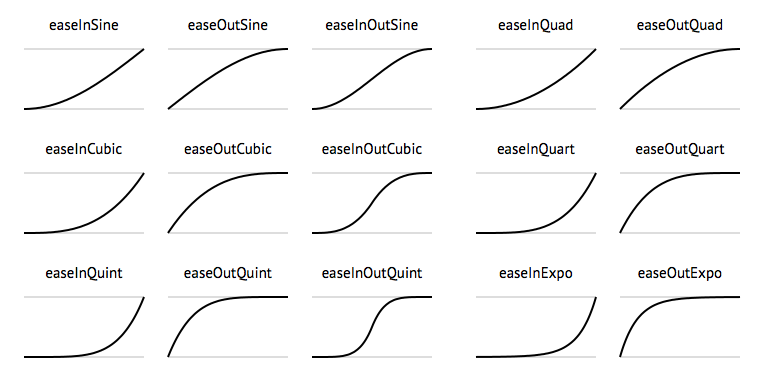
\includegraphics[width=1\textwidth]{easeing}
    \end{subfigure}

    \caption{Funções comumente usadas em interpolações de valores\label{fig:subfigures} (Imagem retirada do artigo de~\cite{VideoGameJuice})}
\end{figure}

O uso de \textit{tweens} se torna extremamente aparente quando utilizamos funções quadráticas, cúbicas, senoidais ou até mesmo elásticas para realizarmos a interpolação. Este efeito pode ser visto, por exemplo, no uso da bomba. Quando uma bomba é utilizada, uma circunferência (efeito da explosão) envolvendo a nave é rapidamente desenhada, tendo seu raio aumentado através de um \textit{tween} baseado em uma função cúbica. Após algumas frações de segundos, o raio da circunferência passa a ser aumentado em uma taxa consideravelmente menor, até finalmente parar e desaparecer, passando assim a imagem de uma explosão para o jogador.

Já não dependendo tanto dos \textit{tweens}, alguns dos \textit{sprites} de balas utilizados no jogos possuem um formato similar a de um losango achatado, com o intuito de clareza quanto à direção em que a bala se move. Balas circulares, por outro lado, podem deixar o entendimento de sua direção mais difícil para o jogador, e por conta disso são utilizadas mais frequentemente por chefes e sub-chefes.

Não se limitando aos visuais, a expressividade do jogo depende também de como os efeitos sonoros são utilizados. Eventos como \textit{ganhar uma vida} e \textit{ganhar uma bomba} são convenientemente demonstrados através de um efeito sonoro curto, distintos entre si, podendo também ser acompanhados de um pequeno indicador visual acima da nave. Neste caso, o \textit{tweening} também se mostra conveniente para suavizar a animação do texto (algo como \textit{Life up!} ou \textit{Bomb get!}) para cima e tornar o evento menos engessado.

% indicadores de qualquer coisa, mencionar a dificuldade depois só

% Variações em tempo real dos visuais gerais do jogo podem se mostrar úteis para indicação 
\par

%!TeX root=../tese.tex
%("dica" para o editor de texto: este arquivo é parte de um documento maior)
% para saber mais: https://tex.stackexchange.com/q/78101/183146

%% ------------------------------------------------------------------------- %%
\chapter{Plataforma de Desenvolvimento}
\label{cap:plataforma de desenvolvimento}
\section{Ideias Iniciais}


\par

%!TeX root=../tese.tex
%("dica" para o editor de texto: este arquivo é parte de um documento maior)
% para saber mais: https://tex.stackexchange.com/q/78101/183146

%% ------------------------------------------------------------------------- %%
\chapter{Balanceamento Dinâmico}
\label{cap:balanceamento dinamico}
\section{Interpretação de Ações}


\par


% Os capítulos de compõem a dissertação/tese, com numeração normal, podem
% ser inseridos diretamente aqui ou "puxados" de outros arquivos.
% Em alguns (raros) casos, pode ser interessante usar \include ao
% invés de \input: https://tex.stackexchange.com/a/32058/183146

%\input{conteudo/01...}
%\par

%\input{conteudo/02...}
%\par
